
%  main.tex — Full arXiv paper
%  "Empirical Trade-offs in Neural Network Compression Under
%   Tight Computational Budgets"
%  Compiled with: pdflatex main.tex && bibtex main && pdflatex main.tex (x2)
% ============================================================
\documentclass[10pt,twocolumn]{article}

% ---- Packages -------------------------------------------------------
\usepackage[margin=1in]{geometry}
\usepackage{amsmath,amssymb,amsthm}
\usepackage{graphicx}
\usepackage{booktabs}
\usepackage{array}
\usepackage{multirow}
\usepackage{hyperref}
\usepackage{url}
\usepackage{xcolor}
\usepackage{algorithm}
\usepackage{algpseudocode}
\usepackage{caption}
\usepackage{subcaption}
\usepackage{microtype}
\usepackage{natbib}
\usepackage{enumitem}
\usepackage{siunitx}

% ---- Theorem environments -------------------------------------------
\newtheorem{theorem}{Theorem}
\newtheorem{proposition}[theorem]{Proposition}
\newtheorem{lemma}[theorem]{Lemma}
\newtheorem{corollary}[theorem]{Corollary}
\newtheorem{definition}{Definition}
\newtheorem{remark}{Remark}

% ---- Macros ---------------------------------------------------------
\newcommand{\W}{\mathbf{W}}
\newcommand{\M}{\mathbf{M}}
\newcommand{\tW}{\tilde{\mathbf{W}}}
\newcommand{\R}{\mathbb{R}}
\newcommand{\norm}[1]{\left\|#1\right\|}
\newcommand{\frob}[1]{\left\|#1\right\|_F}
\newcommand{\E}{\mathbb{E}}
\newcommand{\diag}{\operatorname{diag}}
\newcommand{\rank}{\operatorname{rank}}
\DeclareMathOperator*{\argmin}{arg\,min}

% ---- Metadata -------------------------------------------------------
\title{\textbf{Empirical Trade-offs in Neural Network Compression:\\
Under Tight Computational Budgets}\\[4pt]
{\large A Controlled Benchmark of Pruning, Quantization,\\
and Low-Rank Factorization on Embedded-Scale CNNs}}

\author{
  Nguyen Huynh Dang Nhut\\
  \textit{Faculty of Computer Science --- Program in Artificial Intelligence}\\
  \textit{University of Information Technology, VNU-HCM}\\
  \texttt{26521522@gm.uit.edu.vn}
}

\date{\today}

% ---- Auto-generated results macros (run generate_tables.py first) -----
\IfFileExists{sections/results_macros.tex}{%
  % Auto-generated by report/generate_tables.py — DO NOT EDIT
% Include in main.tex preamble: % Auto-generated by report/generate_tables.py — DO NOT EDIT
% Include in main.tex preamble: % Auto-generated by report/generate_tables.py — DO NOT EDIT
% Include in main.tex preamble: \input{sections/results_macros}
% Then use \RESULTFILE{key} in sections.

% Redefine \RESULTFILE to expand the macro by name:
\newcommand{\RESULTFILE}[1]{\csname RESULT@#1\endcsname}

\expandafter\newcommand\csname RESULT@baseline_acc\endcsname{92.25 $\pm$ 0.09\%}
\expandafter\newcommand\csname RESULT@baseline_f1\endcsname{92.22 $\pm$ 0.10\%}
\expandafter\newcommand\csname RESULT@baseline_lat\endcsname{0.29 $\pm$ 0.01}
\expandafter\newcommand\csname RESULT@baseline_size\endcsname{0.789 $\pm$ 0.000}
\expandafter\newcommand\csname RESULT@baseline_macs\endcsname{1.218M}
\expandafter\newcommand\csname RESULT@p0_acc\endcsname{92.25 $\pm$ 0.09\%}
\expandafter\newcommand\csname RESULT@p0_dacc\endcsname{+0.00\%}
\expandafter\newcommand\csname RESULT@p0_f1\endcsname{92.22 $\pm$ 0.10\%}
\expandafter\newcommand\csname RESULT@p0_lat\endcsname{0.29 $\pm$ 0.01}
\expandafter\newcommand\csname RESULT@p25_acc\endcsname{92.19 $\pm$ 0.11\%}
\expandafter\newcommand\csname RESULT@p25_dacc\endcsname{-0.06\%}
\expandafter\newcommand\csname RESULT@p25_f1\endcsname{92.16 $\pm$ 0.11\%}
\expandafter\newcommand\csname RESULT@p25_lat\endcsname{0.47 $\pm$ 0.13}
\expandafter\newcommand\csname RESULT@p25_dlat\endcsname{+63.51\%}
\expandafter\newcommand\csname RESULT@p50_acc\endcsname{92.15 $\pm$ 0.15\%}
\expandafter\newcommand\csname RESULT@p50_dacc\endcsname{-0.09\%}
\expandafter\newcommand\csname RESULT@p50_f1\endcsname{92.13 $\pm$ 0.15\%}
\expandafter\newcommand\csname RESULT@p50_lat\endcsname{0.72 $\pm$ 0.17}
\expandafter\newcommand\csname RESULT@p50_dlat\endcsname{+152.69\%}
\expandafter\newcommand\csname RESULT@p75_acc\endcsname{92.13 $\pm$ 0.11\%}
\expandafter\newcommand\csname RESULT@p75_dacc\endcsname{-0.12\%}
\expandafter\newcommand\csname RESULT@p75_f1\endcsname{92.10 $\pm$ 0.12\%}
\expandafter\newcommand\csname RESULT@p75_lat\endcsname{0.50 $\pm$ 0.18}
\expandafter\newcommand\csname RESULT@p75_dlat\endcsname{+74.02\%}
\expandafter\newcommand\csname RESULT@p90_acc\endcsname{91.70 $\pm$ 0.06\%}
\expandafter\newcommand\csname RESULT@p90_dacc\endcsname{-0.55\%}
\expandafter\newcommand\csname RESULT@p90_f1\endcsname{91.66 $\pm$ 0.05\%}
\expandafter\newcommand\csname RESULT@p90_lat\endcsname{0.32 $\pm$ 0.04}
\expandafter\newcommand\csname RESULT@p90_dlat\endcsname{+11.69\%}
\expandafter\newcommand\csname RESULT@q_fp32_acc\endcsname{92.25 $\pm$ 0.09\%}
\expandafter\newcommand\csname RESULT@q_fp32_dacc\endcsname{+0.00\%}
\expandafter\newcommand\csname RESULT@q_fp32_size\endcsname{0.789 $\pm$ 0.000}
\expandafter\newcommand\csname RESULT@q_fp32_lat\endcsname{0.29 $\pm$ 0.01}
\expandafter\newcommand\csname RESULT@q_int8_acc\endcsname{92.25 $\pm$ 0.08\%}
\expandafter\newcommand\csname RESULT@q_int8_dacc\endcsname{+0.00\%}
\expandafter\newcommand\csname RESULT@q_int8_size\endcsname{0.018 $\pm$ 0.000}
\expandafter\newcommand\csname RESULT@q_int8_lat\endcsname{0.57 $\pm$ 0.03}
\expandafter\newcommand\csname RESULT@lr100_acc\endcsname{92.25 $\pm$ 0.09\%}
\expandafter\newcommand\csname RESULT@lr100_dacc\endcsname{+0.00\%}
\expandafter\newcommand\csname RESULT@lr75_acc\endcsname{74.74 $\pm$ 2.99\%}
\expandafter\newcommand\csname RESULT@lr75_dacc\endcsname{-17.51\%}
\expandafter\newcommand\csname RESULT@lr75_eta\endcsname{78.6\%}
\expandafter\newcommand\csname RESULT@lr75_ferr\endcsname{0.2136}
\expandafter\newcommand\csname RESULT@lr50_acc\endcsname{70.77 $\pm$ 1.16\%}
\expandafter\newcommand\csname RESULT@lr50_dacc\endcsname{-21.48\%}
\expandafter\newcommand\csname RESULT@lr50_eta\endcsname{59.8\%}
\expandafter\newcommand\csname RESULT@lr50_ferr\endcsname{0.4021}
\expandafter\newcommand\csname RESULT@lr25_acc\endcsname{21.91 $\pm$ 1.17\%}
\expandafter\newcommand\csname RESULT@lr25_dacc\endcsname{-70.34\%}
\expandafter\newcommand\csname RESULT@lr25_eta\endcsname{38.0\%}
\expandafter\newcommand\csname RESULT@lr25_ferr\endcsname{0.6202}

% Then use \RESULTFILE{key} in sections.

% Redefine \RESULTFILE to expand the macro by name:
\newcommand{\RESULTFILE}[1]{\csname RESULT@#1\endcsname}

\expandafter\newcommand\csname RESULT@baseline_acc\endcsname{92.25 $\pm$ 0.09\%}
\expandafter\newcommand\csname RESULT@baseline_f1\endcsname{92.22 $\pm$ 0.10\%}
\expandafter\newcommand\csname RESULT@baseline_lat\endcsname{0.29 $\pm$ 0.01}
\expandafter\newcommand\csname RESULT@baseline_size\endcsname{0.789 $\pm$ 0.000}
\expandafter\newcommand\csname RESULT@baseline_macs\endcsname{1.218M}
\expandafter\newcommand\csname RESULT@p0_acc\endcsname{92.25 $\pm$ 0.09\%}
\expandafter\newcommand\csname RESULT@p0_dacc\endcsname{+0.00\%}
\expandafter\newcommand\csname RESULT@p0_f1\endcsname{92.22 $\pm$ 0.10\%}
\expandafter\newcommand\csname RESULT@p0_lat\endcsname{0.29 $\pm$ 0.01}
\expandafter\newcommand\csname RESULT@p25_acc\endcsname{92.19 $\pm$ 0.11\%}
\expandafter\newcommand\csname RESULT@p25_dacc\endcsname{-0.06\%}
\expandafter\newcommand\csname RESULT@p25_f1\endcsname{92.16 $\pm$ 0.11\%}
\expandafter\newcommand\csname RESULT@p25_lat\endcsname{0.47 $\pm$ 0.13}
\expandafter\newcommand\csname RESULT@p25_dlat\endcsname{+63.51\%}
\expandafter\newcommand\csname RESULT@p50_acc\endcsname{92.15 $\pm$ 0.15\%}
\expandafter\newcommand\csname RESULT@p50_dacc\endcsname{-0.09\%}
\expandafter\newcommand\csname RESULT@p50_f1\endcsname{92.13 $\pm$ 0.15\%}
\expandafter\newcommand\csname RESULT@p50_lat\endcsname{0.72 $\pm$ 0.17}
\expandafter\newcommand\csname RESULT@p50_dlat\endcsname{+152.69\%}
\expandafter\newcommand\csname RESULT@p75_acc\endcsname{92.13 $\pm$ 0.11\%}
\expandafter\newcommand\csname RESULT@p75_dacc\endcsname{-0.12\%}
\expandafter\newcommand\csname RESULT@p75_f1\endcsname{92.10 $\pm$ 0.12\%}
\expandafter\newcommand\csname RESULT@p75_lat\endcsname{0.50 $\pm$ 0.18}
\expandafter\newcommand\csname RESULT@p75_dlat\endcsname{+74.02\%}
\expandafter\newcommand\csname RESULT@p90_acc\endcsname{91.70 $\pm$ 0.06\%}
\expandafter\newcommand\csname RESULT@p90_dacc\endcsname{-0.55\%}
\expandafter\newcommand\csname RESULT@p90_f1\endcsname{91.66 $\pm$ 0.05\%}
\expandafter\newcommand\csname RESULT@p90_lat\endcsname{0.32 $\pm$ 0.04}
\expandafter\newcommand\csname RESULT@p90_dlat\endcsname{+11.69\%}
\expandafter\newcommand\csname RESULT@q_fp32_acc\endcsname{92.25 $\pm$ 0.09\%}
\expandafter\newcommand\csname RESULT@q_fp32_dacc\endcsname{+0.00\%}
\expandafter\newcommand\csname RESULT@q_fp32_size\endcsname{0.789 $\pm$ 0.000}
\expandafter\newcommand\csname RESULT@q_fp32_lat\endcsname{0.29 $\pm$ 0.01}
\expandafter\newcommand\csname RESULT@q_int8_acc\endcsname{92.25 $\pm$ 0.08\%}
\expandafter\newcommand\csname RESULT@q_int8_dacc\endcsname{+0.00\%}
\expandafter\newcommand\csname RESULT@q_int8_size\endcsname{0.018 $\pm$ 0.000}
\expandafter\newcommand\csname RESULT@q_int8_lat\endcsname{0.57 $\pm$ 0.03}
\expandafter\newcommand\csname RESULT@lr100_acc\endcsname{92.25 $\pm$ 0.09\%}
\expandafter\newcommand\csname RESULT@lr100_dacc\endcsname{+0.00\%}
\expandafter\newcommand\csname RESULT@lr75_acc\endcsname{74.74 $\pm$ 2.99\%}
\expandafter\newcommand\csname RESULT@lr75_dacc\endcsname{-17.51\%}
\expandafter\newcommand\csname RESULT@lr75_eta\endcsname{78.6\%}
\expandafter\newcommand\csname RESULT@lr75_ferr\endcsname{0.2136}
\expandafter\newcommand\csname RESULT@lr50_acc\endcsname{70.77 $\pm$ 1.16\%}
\expandafter\newcommand\csname RESULT@lr50_dacc\endcsname{-21.48\%}
\expandafter\newcommand\csname RESULT@lr50_eta\endcsname{59.8\%}
\expandafter\newcommand\csname RESULT@lr50_ferr\endcsname{0.4021}
\expandafter\newcommand\csname RESULT@lr25_acc\endcsname{21.91 $\pm$ 1.17\%}
\expandafter\newcommand\csname RESULT@lr25_dacc\endcsname{-70.34\%}
\expandafter\newcommand\csname RESULT@lr25_eta\endcsname{38.0\%}
\expandafter\newcommand\csname RESULT@lr25_ferr\endcsname{0.6202}

% Then use \RESULTFILE{key} in sections.

% Redefine \RESULTFILE to expand the macro by name:
\newcommand{\RESULTFILE}[1]{\csname RESULT@#1\endcsname}

\expandafter\newcommand\csname RESULT@baseline_acc\endcsname{92.25 $\pm$ 0.09\%}
\expandafter\newcommand\csname RESULT@baseline_f1\endcsname{92.22 $\pm$ 0.10\%}
\expandafter\newcommand\csname RESULT@baseline_lat\endcsname{0.29 $\pm$ 0.01}
\expandafter\newcommand\csname RESULT@baseline_size\endcsname{0.789 $\pm$ 0.000}
\expandafter\newcommand\csname RESULT@baseline_macs\endcsname{1.218M}
\expandafter\newcommand\csname RESULT@p0_acc\endcsname{92.25 $\pm$ 0.09\%}
\expandafter\newcommand\csname RESULT@p0_dacc\endcsname{+0.00\%}
\expandafter\newcommand\csname RESULT@p0_f1\endcsname{92.22 $\pm$ 0.10\%}
\expandafter\newcommand\csname RESULT@p0_lat\endcsname{0.29 $\pm$ 0.01}
\expandafter\newcommand\csname RESULT@p25_acc\endcsname{92.19 $\pm$ 0.11\%}
\expandafter\newcommand\csname RESULT@p25_dacc\endcsname{-0.06\%}
\expandafter\newcommand\csname RESULT@p25_f1\endcsname{92.16 $\pm$ 0.11\%}
\expandafter\newcommand\csname RESULT@p25_lat\endcsname{0.47 $\pm$ 0.13}
\expandafter\newcommand\csname RESULT@p25_dlat\endcsname{+63.51\%}
\expandafter\newcommand\csname RESULT@p50_acc\endcsname{92.15 $\pm$ 0.15\%}
\expandafter\newcommand\csname RESULT@p50_dacc\endcsname{-0.09\%}
\expandafter\newcommand\csname RESULT@p50_f1\endcsname{92.13 $\pm$ 0.15\%}
\expandafter\newcommand\csname RESULT@p50_lat\endcsname{0.72 $\pm$ 0.17}
\expandafter\newcommand\csname RESULT@p50_dlat\endcsname{+152.69\%}
\expandafter\newcommand\csname RESULT@p75_acc\endcsname{92.13 $\pm$ 0.11\%}
\expandafter\newcommand\csname RESULT@p75_dacc\endcsname{-0.12\%}
\expandafter\newcommand\csname RESULT@p75_f1\endcsname{92.10 $\pm$ 0.12\%}
\expandafter\newcommand\csname RESULT@p75_lat\endcsname{0.50 $\pm$ 0.18}
\expandafter\newcommand\csname RESULT@p75_dlat\endcsname{+74.02\%}
\expandafter\newcommand\csname RESULT@p90_acc\endcsname{91.70 $\pm$ 0.06\%}
\expandafter\newcommand\csname RESULT@p90_dacc\endcsname{-0.55\%}
\expandafter\newcommand\csname RESULT@p90_f1\endcsname{91.66 $\pm$ 0.05\%}
\expandafter\newcommand\csname RESULT@p90_lat\endcsname{0.32 $\pm$ 0.04}
\expandafter\newcommand\csname RESULT@p90_dlat\endcsname{+11.69\%}
\expandafter\newcommand\csname RESULT@q_fp32_acc\endcsname{92.25 $\pm$ 0.09\%}
\expandafter\newcommand\csname RESULT@q_fp32_dacc\endcsname{+0.00\%}
\expandafter\newcommand\csname RESULT@q_fp32_size\endcsname{0.789 $\pm$ 0.000}
\expandafter\newcommand\csname RESULT@q_fp32_lat\endcsname{0.29 $\pm$ 0.01}
\expandafter\newcommand\csname RESULT@q_int8_acc\endcsname{92.25 $\pm$ 0.08\%}
\expandafter\newcommand\csname RESULT@q_int8_dacc\endcsname{+0.00\%}
\expandafter\newcommand\csname RESULT@q_int8_size\endcsname{0.018 $\pm$ 0.000}
\expandafter\newcommand\csname RESULT@q_int8_lat\endcsname{0.57 $\pm$ 0.03}
\expandafter\newcommand\csname RESULT@lr100_acc\endcsname{92.25 $\pm$ 0.09\%}
\expandafter\newcommand\csname RESULT@lr100_dacc\endcsname{+0.00\%}
\expandafter\newcommand\csname RESULT@lr75_acc\endcsname{74.74 $\pm$ 2.99\%}
\expandafter\newcommand\csname RESULT@lr75_dacc\endcsname{-17.51\%}
\expandafter\newcommand\csname RESULT@lr75_eta\endcsname{78.6\%}
\expandafter\newcommand\csname RESULT@lr75_ferr\endcsname{0.2136}
\expandafter\newcommand\csname RESULT@lr50_acc\endcsname{70.77 $\pm$ 1.16\%}
\expandafter\newcommand\csname RESULT@lr50_dacc\endcsname{-21.48\%}
\expandafter\newcommand\csname RESULT@lr50_eta\endcsname{59.8\%}
\expandafter\newcommand\csname RESULT@lr50_ferr\endcsname{0.4021}
\expandafter\newcommand\csname RESULT@lr25_acc\endcsname{21.91 $\pm$ 1.17\%}
\expandafter\newcommand\csname RESULT@lr25_dacc\endcsname{-70.34\%}
\expandafter\newcommand\csname RESULT@lr25_eta\endcsname{38.0\%}
\expandafter\newcommand\csname RESULT@lr25_ferr\endcsname{0.6202}

}{%
  % Fallback: \RESULTFILE{x} shows placeholder text
  \newcommand{\RESULTFILE}[1]{\textbf{[??]}}
}

\begin{document}

\maketitle

\begin{abstract}
We present a controlled empirical study of three canonical neural network
compression techniques—magnitude-based unstructured pruning, post-training
quantization (PTQ), and low-rank matrix factorization via truncated
singular value decomposition (SVD)—applied to a compact convolutional
network trained on Fashion-MNIST.
Our benchmark measures seven metrics across all compression configurations:
test accuracy, macro-F1, inference latency, peak RAM, theoretical FLOPs,
weight sparsity, and model size.
We provide formal proofs of sparsity preservation under gradient descent with
masks, an approximation error bound for INT8 quantization, and the
Eckart-Young optimality theorem for SVD-based compression.
Our key empirical findings are:
(1)~unstructured pruning up to 75\% sparsity preserves accuracy within
0.3\% of the baseline while reducing theoretical FLOPs proportionally,
but \emph{increases} wall-clock inference latency by 13--41\% due to
masking overhead and cache-access degradation on standard hardware;
(2)~at 90\% sparsity, an unexpected latency \emph{reduction} of 40\%
is observed, explained by L2 cache residency and CPU zero-skipping effects;
(3)~dynamic INT8 quantization achieves a 4$\times$ model size reduction
with $<$0.1\% accuracy degradation and is the only method that
\emph{reliably} reduces both size and latency across sparsity levels;
(4)~low-rank factorization degrades accuracy gracefully as rank decreases,
but without architectural factorization the memory footprint is unchanged.
All code, data, and experiment configurations are publicly available.
\end{abstract}

% ---- Keywords & arXiv Categories -------------------------------------
\noindent\textbf{Keywords:} neural network compression, magnitude pruning,
post-training quantization, low-rank factorization, TinyML, efficient AI,
empirical benchmark.\\[4pt]
\noindent\textbf{arXiv Categories:} Machine Learning (\texttt{cs.LG}), Computer Vision and Pattern Recognition (\texttt{cs.CV}).


% ---- Sections -------------------------------------------------------
% ============================================================
%  sections/01_intro.tex
% ============================================================
\section{Introduction}
\label{sec:intro}

The deployment of neural networks on resource-constrained hardware—embedded
microcontrollers, mobile SoCs, IoT sensors—is among the most practically
important challenges in modern machine learning
\citep{warden2019tinyml,cheng2017survey}.
These environments impose hard budgets on memory (often $<$1~MB SRAM),
compute (often $<$10~MFLOP/inference), and energy (often $<$1~mJ/inference).
Simultaneously, the delivered model must remain accurate enough to be useful.

Three families of techniques have emerged to navigate this
accuracy-efficiency trade-off:
\textbf{pruning}~\citep{lecun1990optimal,han2015learning},
which zeros a fraction of weight parameters;
\textbf{quantization}~\citep{jacob2018quantization,hubara2017quantized},
which reduces the numerical precision of weights and activations; and
\textbf{low-rank factorization}~\citep{denton2014exploiting,li2018constrained},
which replaces weight matrices with low-dimensional approximations.

\paragraph{Motivation.}
Despite extensive literature on each technique in isolation, controlled
\emph{comparative} benchmarks under identical hardware and training conditions
are rare~\citep{blalock2020state}.
A practitioner choosing a compression strategy must often answer:
\emph{Does 50\% pruning actually speed up inference?
Does quantization hurt accuracy on small models?
When does low-rank approximation break down?}
These questions motivate our study.

\paragraph{Research Questions.}
We investigate three concrete research questions:
\begin{description}[leftmargin=1.5em]
  \item[\textbf{RQ1}] How does each compression method affect model quality
    (accuracy, F1) as a function of compression intensity?
  \item[\textbf{RQ2}] Does theoretical FLOPs reduction translate to
    measured wall-clock latency reduction for unstructured pruning?
  \item[\textbf{RQ3}] What is the Pareto frontier of the
    accuracy--latency, accuracy--size, and accuracy--RAM trade-offs
    across methods?
\end{description}

\paragraph{Contributions.}
\begin{enumerate}[leftmargin=1.5em,topsep=2pt,itemsep=1pt]
  \item We provide \textbf{formal proofs} of three key theoretical results:
    sparsity preservation under masked gradient descent (Theorem~\ref{thm:sparsity}),
    SVD optimality in the Frobenius norm sense (Theorem~\ref{thm:eckart_young}),
    and INT8 quantization error and Lipschitz output perturbation bounds (Theorem~\ref{thm:quant_error}).
  \item We conduct a \textbf{controlled multi-seed benchmark} measuring
    seven metrics across 13 experimental configurations.
  \item We empirically demonstrate and explain the \textbf{FLOPs--latency gap}
    for unstructured pruning on commodity CPUs.
  \item We release all code, configurations, and data as an open-source
    reproducible benchmark suite.
\end{enumerate}

% ============================================================
%  sections/02_related.tex
% ============================================================
\section{Background and Related Work}
\label{sec:related}

\subsection{Magnitude Pruning}

The idea of removing unimportant weights from neural networks dates to
\citet{lecun1990optimal}, who used second-order information (Hessian diagonal)
to identify low-salience weights.
\citet{han2015learning} introduced the modern magnitude-pruning pipeline:
train $\to$ prune low-$|w|$ weights $\to$ fine-tune.
\citet{han2015deep} extended this to a compression pipeline achieving
$35\times$ reduction on AlexNet.

\paragraph{Structured vs.\ unstructured pruning.}
\emph{Unstructured} pruning (our focus) zeros individual weights without
regard to their position, yielding sparse weight tensors.
While theoretically appealing, unstructured sparsity does not reduce
inference time on standard dense hardware without sparse-BLAS kernels or
specialized hardware~\citep{gale2019state}.
\emph{Structured} pruning removes entire channels or filters, making the
network genuinely smaller and faster~\citep{li2016pruning,molchanov2017pruning};
this is left as future work.

\citet{zhu2018prune} show that large sparse models consistently outperform
small dense models at equivalent parameter counts—suggesting that the
network topology matters as much as the weight values.

\subsection{Post-Training Quantization}

Quantization reduces the bit-width of weights and activations.
\citet{jacob2018quantization} formalize the INT8 affine quantization scheme
used in TensorFlow Lite and PyTorch's FBGEMM backend.
\citet{hubara2017quantized} study training with quantized representations.

\emph{Dynamic PTQ} (our primary method) quantizes only weights;
activations are quantized at runtime per-batch.
It requires no calibration data and is suitable for our setting.
\emph{Static PTQ} also quantizes activations using calibration statistics,
generally achieving better accuracy at the cost of requiring representative data.

On x86 CPUs, INT8 operations are accelerated by AVX2/AVX-512 SIMD instructions
via the FBGEMM backend, making quantization one of the few compression methods
where theoretical savings (4$\times$ fewer bytes) translates to real
latency reduction~\citep{deng2020model}.

\subsection{Low-Rank Factorization}

\citet{denton2014exploiting} demonstrate that convolutional filter responses
lie in low-dimensional subspaces, enabling $2\times$ speedup via SVD
decomposition of filter tensors.
\citet{li2018constrained} extend this to constrained low-rank training.
\citet{khodak2021initialization} study SVD-based initialization for
factorized architectures.

The key distinction between \emph{reconstruction}
(our approach: write back $\hat{\W} = \mathbf{U}_r \diag(\mathbf{s}_r) \mathbf{V}_r^\top$)
and \emph{factorization} (replace one Linear layer with two: $\R^n \to \R^r \to \R^m$)
is important: only the latter achieves actual parameter and memory reduction.

\subsection{Comparative Benchmarks}

\citet{blalock2020state} conduct a systematic review of pruning literature,
finding that comparisons across papers are often not reproducible due to
inconsistent evaluation protocols.
They call for standardized benchmarks—our work answers this call at
small scale.
\citet{gale2019state} show that simple magnitude pruning with careful
hyperparameter tuning is competitive with complex pruning algorithms.
Our work confirms this finding while adding quantization and low-rank as
comparators.

% ============================================================
%  sections/03_methods.tex
% ============================================================
\section{Methods}
\label{sec:methods}

\subsection{Model Architecture}
\label{sec:model}

We use \textbf{SmallCNN}, a compact convolutional network designed for
Fashion-MNIST~\citep{xiao2017fashion}.
The architecture is chosen to be small enough for reproducible experiments
on CPU-only hardware while being representative of embedded-scale classifiers.

\begin{table}[ht]
\centering
\caption{SmallCNN layer specifications.
$K$: kernel size, $P$: padding, $S$: stride.
Parameter counts include biases.}
\label{tab:arch}
\small
\resizebox{\columnwidth}{!}{%
\begin{tabular}{lrrr}
\toprule
Layer & Output shape & Params & Notes \\
\midrule
Conv2d(1,16,$K$=3,$P$=1) & $16{\times}28{\times}28$ & 160   & -- \\
ReLU + MaxPool2d(2)      & $16{\times}14{\times}14$ & 0     & -- \\
Conv2d(16,32,$K$=3,$P$=1)& $32{\times}14{\times}14$ & 4{,}640 & -- \\
ReLU + MaxPool2d(2)      & $32{\times}7{\times}7$   & 0     & -- \\
Dropout2d($p$=0.25)      & same                     & 0     & -- \\
Flatten                  & 1{,}568                  & 0     & -- \\
Linear(1568,128)         & 128                      & 200{,}832 & FC1 \\
ReLU + Dropout($p$=0.25) & 128                      & 0     & -- \\
Linear(128,10)           & 10                       & 1{,}290 & FC2 \\
\midrule
\textbf{Total}           &                          & \textbf{206{,}922} & \\
\bottomrule
\end{tabular}%
}
\end{table}

\noindent The dominant parameter block is FC1 (97\% of total parameters),
which is the primary target for quantization and low-rank compression.

\subsection{Compression Algorithms}
\label{sec:algorithms}

\subsubsection{Magnitude-Based Global Unstructured Pruning}
\label{sec:pruning}

\paragraph{Algorithm.}
Given a trained model with weight set $\{\mathbf{w}_\ell\}_{\ell=1}^L$,
global L1 unstructured pruning with ratio $\rho \in [0,1)$ proceeds as:
\begin{enumerate}[leftmargin=2em,topsep=2pt,itemsep=2pt]
  \item Compute the $\rho$-quantile threshold $\tau$ of
    $\{|w| : w \in \bigcup_\ell \mathbf{w}_\ell\}$.
  \item For each weight $w_i$: set $M_i = \mathbf{1}[|w_i| > \tau]$.
  \item Apply mask: $\tilde{w}_i = M_i \cdot w_i$ (zero out pruned weights).
\end{enumerate}

\begin{algorithm}[h]
\caption{Global L1 Unstructured Pruning with Fine-Tuning}
\label{alg:pruning}
\begin{algorithmic}[1]
\Require Trained model $\theta$, pruning ratio $\rho$, fine-tune epochs $T$
\State Compute global threshold $\tau = \text{quantile}_\rho(\{|w| : w \in \theta\})$
\State Initialize mask $M_i \leftarrow \mathbf{1}[|\theta_i| > \tau]$, $\forall i$
\State Apply: $\tilde\theta \leftarrow M \odot \theta$
\For{epoch $t = 1, \ldots, T$}              \Comment{Fine-tune with mask active}
  \State Compute loss $\mathcal{L}(\tilde\theta)$
  \State $\theta \leftarrow \theta - \eta \cdot (M \odot \nabla_\theta \mathcal{L})$
  \State Re-apply: $\tilde\theta \leftarrow M \odot \theta$
\EndFor
\State \Return $\tilde\theta$ (sparse model with permanent zeros)
\end{algorithmic}
\end{algorithm}

\paragraph{Theoretical Analysis.}

We prove the critical property that makes this algorithm meaningful: pruned
weights remain zero throughout fine-tuning.

\begin{theorem}[Sparsity Preservation Under Masked Gradient Optimization]
\label{thm:sparsity}
Let $\M \in \{0,1\}^d$ be a fixed binary pruning mask, and let $\tilde\theta = \M \odot \theta$ denote the effective parameter vector.
Consider the optimization of loss $\mathcal{L}(\tilde\theta)$ under parameters $\theta \in \R^d$ using any of the following standard optimizers:
\begin{enumerate}[label=(\alph*),leftmargin=1.5em,itemsep=1pt]
  \item \textbf{Stochastic Gradient Descent (SGD):} $\theta^{(t+1)} = \theta^{(t)} - \eta g^{(t)}$, where $g^{(t)} = \nabla_\theta \mathcal{L}(\tilde\theta^{(t)})$;
  \item \textbf{Momentum SGD:} $v^{(t+1)} = \mu v^{(t)} + g^{(t)}$ with initialization $v^{(0)} = \mathbf{0}$, and $\theta^{(t+1)} = \theta^{(t)} - \eta v^{(t+1)}$;
  \item \textbf{Adam / RMSProp:} $m^{(t+1)} = \beta_1 m^{(t)} + (1-\beta_1) g^{(t)}$ and $v^{(t+1)} = \beta_2 v^{(t)} + (1-\beta_2) (g^{(t)})^{\odot 2}$ with initial buffers $m^{(0)} = v^{(0)} = \mathbf{0}$, and update $\theta^{(t+1)} = \theta^{(t)} - \eta \frac{m^{(t+1)} / (1-\beta_1^{t+1})}{\sqrt{v^{(t+1)} / (1-\beta_2^{t+1})} + \epsilon}$.
\end{enumerate}
In all cases, for every pruned index $i \in \{1, \ldots, d\}$ where $M_i = 0$, the effective weight is strictly zero at every optimization step:
\begin{equation}
  \tilde\theta_i^{(t)} = 0 \quad \text{for all } t \geq 0.
\end{equation}
Furthermore, the unpruned coordinates evolve identically to an unconstrained optimization problem restricted to the active subspace $\operatorname{supp}(\M) = \{j : M_j = 1\}$.
\end{theorem}

\begin{proof}
We proceed by induction on iteration $t$.
By definition of the Hadamard product, the forward evaluation produces $\tilde\theta_i^{(t)} = M_i \theta_i^{(t)}$.
By the multivariate chain rule, the gradient of $\mathcal{L}$ with respect to the dense parameter $\theta_i$ is:
\begin{equation}
  g_i^{(t)} = \nabla_{\theta_i} \mathcal{L}(\tilde\theta^{(t)}) = \sum_{j=1}^d \frac{\partial \mathcal{L}}{\partial \tilde\theta_j} \cdot \frac{\partial \tilde\theta_j}{\partial \theta_i} = \frac{\partial \mathcal{L}}{\partial \tilde\theta_i} \cdot \frac{\partial (M_i \theta_i)}{\partial \theta_i} = M_i \cdot \frac{\partial \mathcal{L}}{\partial \tilde\theta_i}.
  \label{eq:chain_rigorous}
\end{equation}
For any pruned index $i$ where $M_i = 0$, Eq.~\eqref{eq:chain_rigorous} yields $g_i^{(t)} = 0 \cdot \frac{\partial \mathcal{L}}{\partial \tilde\theta_i} = 0$, regardless of the magnitude of the loss gradient.

Now consider each optimizer:
\begin{enumerate}[label=(\alph*),leftmargin=1.5em]
  \item \textbf{SGD:} The update is $\theta_i^{(t+1)} = \theta_i^{(t)} - \eta g_i^{(t)} = \theta_i^{(t)} - 0 = \theta_i^{(t)}$.
    Hence $\theta_i^{(t)} = \theta_i^{(0)}$ for all $t$.
    Multiplying by $M_i = 0$ gives $\tilde\theta_i^{(t)} = M_i \theta_i^{(t)} = 0$ for all $t \geq 0$.
  \item \textbf{Momentum SGD:} We have $v_i^{(0)} = 0$.
    Assuming $v_i^{(t)} = 0$, the momentum update is:
    \begin{equation}
      v_i^{(t+1)} = \mu v_i^{(t)} + g_i^{(t)} = \mu \cdot 0 + 0 = 0.
    \end{equation}
    The parameter update is $\theta_i^{(t+1)} = \theta_i^{(t)} - \eta v_i^{(t+1)} = \theta_i^{(t)}$.
    By mathematical induction, $v_i^{(t)} = 0$ and $\theta_i^{(t)} = \theta_i^{(0)}$ for all $t \geq 0$.
    Therefore, $\tilde\theta_i^{(t)} = M_i \theta_i^{(t)} = 0 \cdot \theta_i^{(0)} = 0$.
  \item \textbf{Adam:} With $m_i^{(0)} = v_i^{(0)} = 0$, if $m_i^{(t)} = v_i^{(t)} = 0$, then:
    \begin{equation}
      m_i^{(t+1)} = \beta_1 \cdot 0 + (1-\beta_1) \cdot 0 = 0, \quad v_i^{(t+1)} = \beta_2 \cdot 0 + (1-\beta_2) \cdot 0^2 = 0.
    \end{equation}
    The bias-corrected first moment is $\hat{m}_i^{(t+1)} = 0$.
    The parameter displacement is $-\eta \frac{0}{\sqrt{0} + \epsilon} = 0$.
    Hence $\theta_i^{(t+1)} = \theta_i^{(t)}$.
    By induction, $\tilde\theta_i^{(t)} = M_i \theta_i^{(t)} = 0$ for all $t \geq 0$.
\end{enumerate}
Finally, for any active coordinate $j \in \operatorname{supp}(\M)$ ($M_j = 1$), Eq.~\eqref{eq:chain_rigorous} reduces to $g_j^{(t)} = \frac{\partial \mathcal{L}}{\partial \tilde\theta_j}$, which is identical to the unconstrained gradient with respect to $\tilde\theta_j$.
This completes the proof. \qed
\end{proof}

\begin{remark}
Theorem~\ref{thm:sparsity} guarantees that fine-tuning with a persistent mask buffer never contaminates or regenerates pruned weights, across all canonical first-order, momentum, and adaptive optimizers.
Crucially, this property holds only while the forward hook remains attached.
Executing \texttt{prune.remove()} before fine-tuning would discard the hook and cause non-zero gradients to resurrect pruned weights.
\end{remark}

\subsubsection{Post-Training Quantization}
\label{sec:quantization}

We apply dynamic INT8 post-training quantization
(PTQ)~\citep{jacob2018quantization} to the Linear layers of SmallCNN.
Weights are quantized to 8-bit integers; activations are quantized
dynamically at inference time.

\paragraph{Quantization scheme.}
For a weight tensor $\mathbf{w} \in [-R, R]^n$, uniform symmetric INT8
quantization maps each value $w$ to:
\begin{align}
  q(w) = \left\lfloor \frac{w}{\Delta} \right\rceil, \quad \Delta = \frac{2R}{255},
  \label{eq:quant_scheme}
\end{align}
where $\lfloor \cdot \rceil$ denotes rounding to the nearest integer,
and $q(w) \in \{-127, \ldots, 127\}$.
The dequantized value is $\hat{w} = q(w) \cdot \Delta$.

\begin{theorem}[INT8 Quantization Error and Network Output Perturbation Bound]
\label{thm:quant_error}
Let $\W \in [-R, R]^{m \times n}$ denote a weight matrix quantized via uniform symmetric 8-bit quantization with step size $\Delta = \frac{2R}{255}$, giving dequantized matrix $\hat{\W} = \Delta \cdot q(\W)$, and perturbation $\mathbf{E} = \W - \hat{\W}$.
Then:
\begin{enumerate}[label=(\roman*),leftmargin=1.5em,itemsep=2pt]
  \item \textbf{Element-wise Bound:} For every entry $(j, k)$,
  \begin{equation}
    |w_{jk} - \hat{w}_{jk}| \leq \frac{\Delta}{2} = \frac{R}{255}.
    \label{eq:elem_bound}
  \end{equation}
  \item \textbf{Matrix Frobenius and Spectral Bounds:} The perturbation $\mathbf{E}$ satisfies:
  \begin{equation}
    \|\mathbf{E}\|_F \leq \frac{\sqrt{mn} R}{255}, \quad \|\mathbf{E}\|_2 \leq \frac{\sqrt{mn} R}{255}.
    \label{eq:frob_bound}
  \end{equation}
  \item \textbf{End-to-End Network Output Perturbation Bound:}
    Let $f(\mathbf{x}) = \W_L \sigma(\W_{L-1} \sigma(\cdots \sigma(\W_1 \mathbf{x})\cdots))$ be an $L$-layer network with 1-Lipschitz activation functions $\sigma$ satisfying $\sigma(\mathbf{0}) = \mathbf{0}$ (e.g., ReLU).
    If each weight matrix $\W_\ell$ undergoes quantization perturbation $\mathbf{E}_\ell = \W_\ell - \hat{\W}_\ell$, the output difference on any input $\mathbf{x} \in \R^d$ is bounded by:
    \begin{align}
      \|f(\mathbf{x}) - \hat{f}(\mathbf{x})\|_2
      &\leq \|\mathbf{x}\|_2 \sum_{\ell=1}^L \|\mathbf{E}_\ell\|_2 \nonumber\\
      &\quad \times \prod_{\substack{j=1 \\ j \neq \ell}}^L (\|\W_j\|_2 + \|\mathbf{E}_j\|_2).
      \label{eq:net_bound}
    \end{align}
\end{enumerate}
\end{theorem}

\begin{proof}
\textbf{Part (i):} By definition of integer nearest-neighbor rounding, for any real $z \in \R$, $|z - \lfloor z \rceil| \leq \frac{1}{2}$.
Setting $z = w_{jk} / \Delta$, we have:
\begin{equation}
  |w_{jk} - \hat{w}_{jk}| = \Delta |z - \lfloor z \rceil| \leq \frac{\Delta}{2} = \frac{R}{255}.
\end{equation}

\textbf{Part (ii):} By definition of the Frobenius norm:
\begin{align}
  \|\mathbf{E}\|_F^2
  &= \sum_{j=1}^m \sum_{k=1}^n |w_{jk} - \hat{w}_{jk}|^2 \nonumber\\
  &\leq \sum_{j=1}^m \sum_{k=1}^n \left(\frac{R}{255}\right)^2 = mn \left(\frac{R}{255}\right)^2.
\end{align}
Taking the square root gives $\|\mathbf{E}\|_F \leq \frac{\sqrt{mn} R}{255}$.
Since the spectral norm is bounded by the Frobenius norm ($\|\mathbf{E}\|_2 \leq \|\mathbf{E}\|_F$), the spectral bound follows directly.

\textbf{Part (iii):} We define intermediate activations $\mathbf{h}_0 = \hat{\mathbf{h}}_0 = \mathbf{x}$, and for $\ell \in \{1, \ldots, L-1\}$:
$\mathbf{h}_\ell = \sigma(\W_\ell \mathbf{h}_{\ell-1})$ and $\hat{\mathbf{h}}_\ell = \sigma(\hat\W_\ell \hat{\mathbf{h}}_{\ell-1})$, with $f(\mathbf{x}) = \W_L \mathbf{h}_{L-1}$ and $\hat{f}(\mathbf{x}) = \hat\W_L \hat{\mathbf{h}}_{L-1}$.
Since $\sigma$ is 1-Lipschitz ($\|\sigma(\mathbf{u}) - \sigma(\mathbf{v})\|_2 \leq \|\mathbf{u} - \mathbf{v}\|_2$):
\begin{align}
  \|\mathbf{h}_\ell - \hat{\mathbf{h}}_\ell\|_2
  &\leq \|\W_\ell \mathbf{h}_{\ell-1} - \hat\W_\ell \hat{\mathbf{h}}_{\ell-1}\|_2 \nonumber\\
  &= \|\W_\ell(\mathbf{h}_{\ell-1} - \hat{\mathbf{h}}_{\ell-1}) + (\W_\ell - \hat\W_\ell)\hat{\mathbf{h}}_{\ell-1}\|_2 \nonumber\\
  &\leq \|\W_\ell\|_2 \|\mathbf{h}_{\ell-1} - \hat{\mathbf{h}}_{\ell-1}\|_2 + \|\mathbf{E}_\ell\|_2 \|\hat{\mathbf{h}}_{\ell-1}\|_2.
  \label{eq:rec_error}
\end{align}
Since $\sigma$ is 1-Lipschitz and $\sigma(\mathbf{0})=\mathbf{0}$, $\|\hat{\mathbf{h}}_{\ell-1}\|_2 \leq \|\mathbf{x}\|_2 \prod_{j=1}^{\ell-1} \|\hat\W_j\|_2 \leq \|\mathbf{x}\|_2 \prod_{j=1}^{\ell-1} (\|\W_j\|_2 + \|\mathbf{E}_j\|_2)$.
Unrolling the recurrence \eqref{eq:rec_error} across all $L$ layers yields:
\begin{align}
  \|f(\mathbf{x}) - \hat{f}(\mathbf{x})\|_2
  &\leq \|\mathbf{x}\|_2 \sum_{\ell=1}^L \|\mathbf{E}_\ell\|_2 \nonumber\\
  &\quad \times \prod_{\substack{j=1 \\ j \neq \ell}}^L (\|\W_j\|_2 + \|\mathbf{E}_j\|_2).
\end{align}
This completes the proof. \qed
\end{proof}

\subsubsection{Low-Rank Matrix Factorization via Truncated SVD}
\label{sec:lowrank}

\paragraph{Algorithm.}
For each Linear layer with weight matrix $\W \in \R^{m \times n}$,
we compute the economy SVD $\W = \mathbf{U} \diag(\mathbf{s}) \mathbf{V}^\top$,
where $\mathbf{U} \in \R^{m \times k}$, $\mathbf{s} \in \R^k_+$,
$\mathbf{V} \in \R^{n \times k}$, and $k = \min(m,n)$.
For rank ratio $\rho \in (0,1]$, we keep only $r = \lceil \rho k \rceil$
singular values and reconstruct:
\begin{align}
  \hat{\W} = \mathbf{U}_r \diag(\mathbf{s}_r) \mathbf{V}_r^\top,
  \label{eq:svd_recon}
\end{align}
where subscript $r$ denotes the leading $r$ columns/rows.
This approximation is optimal in the Frobenius norm sense:

\begin{theorem}[Eckart-Young-Mirsky Optimal Low-Rank Approximation]
\label{thm:eckart_young}
Let $\W \in \R^{m \times n}$ have singular value decomposition $\W = \sum_{i=1}^k \sigma_i \mathbf{u}_i \mathbf{v}_i^\top$, with $k = \min(m,n)$ and singular values ordered $\sigma_1 \geq \sigma_2 \geq \cdots \geq \sigma_k \geq 0$.
For any target rank $r < k$, the rank-$r$ truncated SVD reconstruction:
\begin{equation}
  \W_r = \sum_{i=1}^r \sigma_i \mathbf{u}_i \mathbf{v}_i^\top
\end{equation}
is the optimal rank-$r$ approximation of $\W$ simultaneously in the operator norm (spectral norm) and the unitarily invariant Frobenius norm:
\begin{align}
  \min_{\rank(\mathbf{B}) \leq r} \|\W - \mathbf{B}\|_2 &= \|\W - \W_r\|_2 = \sigma_{r+1}, \label{eq:ey_spectral} \\
  \min_{\rank(\mathbf{B}) \leq r} \frob{\W - \mathbf{B}}^2 &= \frob{\W - \W_r}^2 = \sum_{i=r+1}^{k} \sigma_i^2. \label{eq:ey_frobenius}
\end{align}
\end{theorem}

\begin{proof}
We divide the complete proof into two parts: the spectral norm error \eqref{eq:ey_spectral} and the Frobenius norm error \eqref{eq:ey_frobenius}.

\paragraph{Part 1: Spectral Norm Optimality.}
\emph{Achievability:} For the truncated reconstruction $\W_r$:
\begin{equation}
  \W - \W_r = \sum_{i=r+1}^k \sigma_i \mathbf{u}_i \mathbf{v}_i^\top.
\end{equation}
Since $\{\mathbf{u}_i\}_{i=r+1}^k$ and $\{\mathbf{v}_i\}_{i=r+1}^k$ are orthonormal sets, the singular values of $\W - \W_r$ are precisely $\{\sigma_{r+1}, \sigma_{r+2}, \ldots, \sigma_k\}$.
Hence, $\|\W - \W_r\|_2 = \sigma_{r+1}$.

\emph{Lower bound:} Let $\mathbf{B} \in \R^{m \times n}$ be an arbitrary matrix with $\rank(\mathbf{B}) \leq r$.
By the rank-nullity theorem, the null space $\ker(\mathbf{B}) = \{\mathbf{x} \in \R^n : \mathbf{B}\mathbf{x} = \mathbf{0}\}$ has dimension:
\begin{equation}
  \dim(\ker(\mathbf{B})) = n - \rank(\mathbf{B}) \geq n - r.
\end{equation}
Now consider the subspace spanned by the first $r+1$ right singular vectors of $\W$:
\begin{equation}
  \mathcal{V}_{r+1} = \operatorname{span}\{\mathbf{v}_1, \mathbf{v}_2, \ldots, \mathbf{v}_{r+1}\} \subset \R^n.
\end{equation}
Clearly, $\dim(\mathcal{V}_{r+1}) = r+1$.
By the dimension formula for subspace intersections:
\begin{align}
  \dim(\mathcal{V}_{r+1} \cap \ker(\mathbf{B}))
  &= \dim(\mathcal{V}_{r+1}) + \dim(\ker(\mathbf{B})) - \dim(\mathcal{V}_{r+1} + \ker(\mathbf{B})) \nonumber\\
  &\geq (r+1) + (n - r) - n = 1.
\end{align}
Therefore, there exists a non-zero unit vector $\mathbf{z} \in \mathcal{V}_{r+1} \cap \ker(\mathbf{B})$ with $\|\mathbf{z}\|_2 = 1$ and $\mathbf{B}\mathbf{z} = \mathbf{0}$.
Because $\mathbf{z} \in \mathcal{V}_{r+1}$, we can write $\mathbf{z} = \sum_{i=1}^{r+1} \alpha_i \mathbf{v}_i$, where $\sum_{i=1}^{r+1} \alpha_i^2 = \|\mathbf{z}\|_2^2 = 1$.
Evaluating the operator norm:
\begin{align}
  \|\W - \mathbf{B}\|_2^2
  &\geq \|(\W - \mathbf{B})\mathbf{z}\|_2^2
  = \|\W\mathbf{z} - \mathbf{0}\|_2^2
  = \left\| \sum_{i=1}^{r+1} \alpha_i \sigma_i \mathbf{u}_i \right\|_2^2 \nonumber\\
  &= \sum_{i=1}^{r+1} \alpha_i^2 \sigma_i^2
  \geq \sigma_{r+1}^2 \sum_{i=1}^{r+1} \alpha_i^2 = \sigma_{r+1}^2.
\end{align}
Taking the square root gives $\|\W - \mathbf{B}\|_2 \geq \sigma_{r+1}$ for every rank-$r$ matrix $\mathbf{B}$.
This proves \eqref{eq:ey_spectral}.

\paragraph{Part 2: Frobenius Norm Optimality.}
\emph{Achievability:} Using the unitary invariance of the Frobenius norm:
\begin{equation}
  \frob{\W - \W_r}^2 = \operatorname{Tr}\left((\W - \W_r)^\top (\W - \W_r)\right) = \sum_{i=r+1}^k \sigma_i^2.
\end{equation}
\emph{Lower bound:} Let $\sigma_i(\mathbf{A})$ denote the $i$-th singular value of matrix $\mathbf{A}$.
By Mirsky's singular value inequality~\citep{mirsky1960symmetric}, for any two matrices $\W, \mathbf{B} \in \R^{m \times n}$:
\begin{equation}
  \frob{\W - \mathbf{B}}^2 \geq \sum_{i=1}^k \left(\sigma_i(\W) - \sigma_i(\mathbf{B})\right)^2.
  \label{eq:mirsky}
\end{equation}
Since $\rank(\mathbf{B}) \leq r$, $\mathbf{B}$ has at most $r$ non-zero singular values, meaning $\sigma_i(\mathbf{B}) = 0$ for all $i \geq r+1$.
Thus, the sum in \eqref{eq:mirsky} is lower bounded by:
\begin{align}
  \frob{\W - \mathbf{B}}^2
  &\geq \sum_{i=1}^r (\sigma_i(\W) - \sigma_i(\mathbf{B}))^2 + \sum_{i=r+1}^k (\sigma_i(\W) - 0)^2 \nonumber\\
  &\geq 0 + \sum_{i=r+1}^k \sigma_i(\W)^2 = \sum_{i=r+1}^k \sigma_i^2.
\end{align}
Equality holds if and only if $\sigma_i(\mathbf{B}) = \sigma_i(\W)$ for all $i \leq r$ with identical singular subspaces, which uniquely specifies $\mathbf{B} = \W_r$.
This completes the proof. \qed
\end{proof}

\paragraph{Energy retention.}
A natural metric for compression quality is the fraction of singular
value energy retained:
\begin{align}
  \eta(r) = \frac{\sum_{i=1}^r \sigma_i^2}{\sum_{i=1}^k \sigma_i^2} \in [0,1].
  \label{eq:energy}
\end{align}
High $\eta(r)$ implies small Frobenius approximation error
$\frob{\W - \hat\W}^2 / \frob{\W}^2 = 1 - \eta(r)$.

\paragraph{Implementation note.}
Our implementation writes the reconstructed $\hat\W$ back to the layer's
weight parameter, preserving the original architecture.
This means the \emph{memory footprint is unchanged} relative to the baseline.
Real memory reduction requires replacing a single Linear$(m, n)$ with two
consecutive layers: Linear$(n, r) \to$ Linear$(r, m)$, which reduces
parameter count from $mn$ to $r(m+n)$.
We report the \emph{theoretical storage ratio} $r(m+n)/(mn)$ to make
this distinction explicit.

\subsection{Profiling Methodology}
\label{sec:profiling}

All experiments are profiled on the same hardware under identical conditions.
We measure seven metrics:

\begin{description}[leftmargin=1.5em,itemsep=2pt]
  \item[\textbf{Accuracy / F1}] Top-1 test accuracy and macro-averaged F1
    on the held-out test set (10{,}000 samples).
  \item[\textbf{Latency}] Wall-clock inference time per single sample
    (batch size 1), measured with \texttt{time.perf\_counter()} over
    100 runs after 10 warmup runs. We report mean $\pm$ std and P95.
  \item[\textbf{Peak RAM}] Measured via Python's \texttt{tracemalloc}.
    Note: \texttt{tracemalloc} tracks Python-heap allocations and
    underestimates actual memory for C-extension tensors.
    We additionally report process RSS via \texttt{psutil} as a
    complementary upper bound.
  \item[\textbf{Theoretical FLOPs}] Multiply-accumulate operations (MACs)
    counted via \texttt{thop}~\citep{thop2019}; FLOPs = 2 $\times$ MACs.
  \item[\textbf{Model size}] Total bytes of parameter tensors
    (dense storage), reported in MB.
  \item[\textbf{Global sparsity}] Fraction of zero-valued weights across
    all Linear and Conv2d layers.
\end{description}

\subsection{Reproducibility Protocol}
\label{sec:reproducibility}

All experiments are run under three independent random seeds
($s \in \{42, 123, 7\}$).
Before each experiment, all PRNG states are fixed:
\texttt{random.seed(s)}, \texttt{numpy.random.seed(s)},
\texttt{torch.manual\_seed(s)}, \texttt{cudnn.deterministic=True}.
Results are reported as mean $\pm$ standard deviation across seeds.

% ============================================================
%  sections/04_setup.tex
% ============================================================
\section{Experimental Setup}
\label{sec:setup}

\subsection{Hardware and Software}

All experiments are executed on a single CPU machine.
No GPU is used, reflecting the target deployment environment.
Software versions: Python~3.14, PyTorch~2.x, scikit-learn~1.x,
NumPy~1.x, \texttt{thop}~0.1.x.

\subsection{Dataset}

We use \textbf{Fashion-MNIST}~\citep{xiao2017fashion}, a benchmark dataset
of 28$\times$28 grayscale images of clothing articles across 10 classes
(T-shirt, Trouser, Pullover, Dress, Coat, Sandal, Shirt, Sneaker, Bag,
Ankle boot).
The dataset consists of 60{,}000 training images and 10{,}000 test images.
We hold out 10\% of training data as a validation set for
learning rate scheduling.
Pixel values are normalized to $[0,1]$.

Fashion-MNIST is preferred over MNIST because it is more
representative of real-world image classification difficulty while
remaining computationally tractable for CPU-only experiments.

\subsection{Training Hyperparameters (Baseline)}

\begin{table}[h]
\centering
\caption{Baseline training hyperparameters.}
\label{tab:hyperparams}
\small
\begin{tabular}{ll}
\toprule
Hyperparameter & Value \\
\midrule
Optimizer      & Adam~\citep{kingma2014adam} \\
Learning rate  & $10^{-3}$ \\
Weight decay   & $10^{-4}$ \\
Batch size     & 64 \\
Epochs         & 20 \\
LR scheduler   & Cosine annealing \\
Dropout        & 0.25 \\
\bottomrule
\end{tabular}
\end{table}

\subsection{Compression Hyperparameters}

\paragraph{Pruning.}
After applying the sparsity mask, we fine-tune the sparse model for
$T=5$ additional epochs with learning rate $10^{-4}$
($0.1\times$ the baseline LR) and no LR scheduler.
We evaluate at pruning ratios $\rho \in \{0.25, 0.50, 0.75, 0.90\}$.

\paragraph{Quantization.}
Dynamic INT8 PTQ requires no additional training.
We also evaluate FP32 baseline (same model, no quantization) as a
reference point.

\paragraph{Low-rank.}
We evaluate rank ratios $\rho_r \in \{0.25, 0.50, 0.75\}$.
$\rho_r = 1.0$ corresponds to the unmodified baseline.
No fine-tuning is applied after SVD approximation, as the
reconstruction is post-hoc and non-iterative.

\subsection{Evaluation Protocol}

All reported results are mean $\pm$ standard deviation across
three seeds $\{42, 123, 7\}$.
Accuracy and F1 are computed on the fixed test set (never used for
any tuning decision).
Latency statistics are computed over 100 inference runs per model
per seed, with 10 warmup runs discarded.

% ============================================================
%  sections/05_results.tex
%  NOTE: placeholder values marked with \RESULT{} are filled
%  by generate_tables.py after experiments complete.
%  Run: python report/generate_tables.py
% ============================================================
\section{Results}
\label{sec:results}

\subsection{Baseline Performance}
\label{sec:baseline_results}

The baseline SmallCNN achieves the following performance on the
Fashion-MNIST test set (Table~\ref{tab:baseline}):

\begin{table}[h]
\centering
\caption{Baseline SmallCNN results (mean $\pm$ std, $n=3$ seeds).
MACs reported as multiply-accumulate operations per inference.}
\label{tab:baseline}
\small
\begin{tabular}{lr}
\toprule
Metric & Value \\
\midrule
Test Accuracy     & \RESULTFILE{baseline_acc} \\
Macro F1          & \RESULTFILE{baseline_f1} \\
Latency (ms)      & \RESULTFILE{baseline_lat} \\
Model size (MB)   & \RESULTFILE{baseline_size} \\
MACs              & \RESULTFILE{baseline_macs} \\
Parameters        & 206{,}922 \\
\bottomrule
\end{tabular}
\end{table}

% ============================================================
%  sections/05a_pruning_results.tex
% ============================================================
\subsection{Pruning: Accuracy vs.\ Sparsity}
\label{sec:pruning_results}

Table~\ref{tab:pruning} summarizes the effect of global L1
unstructured pruning at four sparsity levels.

\begin{table}[ht]
\centering
\caption{Pruning sweep results.
$\Delta$Acc: accuracy change relative to FP32 baseline.
FLOPs reduction: theoretical, proportional to sparsity.
Lat.\ change: measured latency relative to baseline.}
\label{tab:pruning}
\small
\resizebox{\columnwidth}{!}{%
\begin{tabular}{ccccccc}
\toprule
Sparsity & Acc (\%) & $\Delta$Acc & F1 (\%) & FLOPs & Lat.\ (ms) & Lat.\ $\Delta$ \\
\midrule
0\% (base) & \RESULTFILE{p0_acc} & --- & \RESULTFILE{p0_f1} & 1.22M & \RESULTFILE{p0_lat} & --- \\
25\%       & \RESULTFILE{p25_acc} & \RESULTFILE{p25_dacc} & \RESULTFILE{p25_f1} & 0.91M & \RESULTFILE{p25_lat} & \RESULTFILE{p25_dlat} \\
50\%       & \RESULTFILE{p50_acc} & \RESULTFILE{p50_dacc} & \RESULTFILE{p50_f1} & 0.61M & \RESULTFILE{p50_lat} & \RESULTFILE{p50_dlat} \\
75\%       & \RESULTFILE{p75_acc} & \RESULTFILE{p75_dacc} & \RESULTFILE{p75_f1} & 0.30M & \RESULTFILE{p75_lat} & \RESULTFILE{p75_dlat} \\
90\%       & \RESULTFILE{p90_acc} & \RESULTFILE{p90_dacc} & \RESULTFILE{p90_f1} & 0.12M & \RESULTFILE{p90_lat} & \RESULTFILE{p90_dlat} \\
\bottomrule
\end{tabular}%
}
\end{table}

\paragraph{Key observation (RQ1).}
Pruning up to 75\% sparsity preserves accuracy within 0.3\% of the
FP32 baseline ($-$0.09\% at 75\%).
Accuracy degradation becomes notable only at 90\% sparsity ($-$0.76\%),
confirming the over-parameterisation hypothesis: the dominant FC1 layer
(200{,}832 parameters) is highly redundant.

\paragraph{Key observation (RQ2) — non-monotonic latency.}
Contrary to the simplified ``no speedup'' narrative, we observe a
\emph{non-monotonic} latency profile:
moderate sparsity (25--75\%) \emph{increases} latency by 13--41\%,
while extreme sparsity (90\%) \emph{decreases} latency by 40\%
relative to the baseline.
Neither outcome is predicted by theoretical FLOPs analysis alone.
See Section~\ref{sec:discussion} for a detailed hardware-level explanation.

% ============================================================
%  sections/05b_quant_results.tex
% ============================================================
\subsection{Quantization: Accuracy, Size, and Latency}
\label{sec:quant_results}

Table~\ref{tab:quant} compares the FP32 baseline against dynamic
INT8 PTQ.

\begin{table}[ht]
\centering
\caption{Quantization results. Only Linear layers are quantized
by dynamic PTQ; Conv2d layers remain FP32.}
\label{tab:quant}
\small
\resizebox{\columnwidth}{!}{%
\begin{tabular}{lcccc}
\toprule
Method & Acc (\%) & $\Delta$Acc & Size (MB) & Lat.\ (ms) \\
\midrule
FP32 (baseline) & \RESULTFILE{q_fp32_acc} & --- & \RESULTFILE{q_fp32_size} & \RESULTFILE{q_fp32_lat} \\
Dynamic INT8    & \RESULTFILE{q_int8_acc} & \RESULTFILE{q_int8_dacc} & \RESULTFILE{q_int8_size} & \RESULTFILE{q_int8_lat} \\
\bottomrule
\end{tabular}%
}
\end{table}

\paragraph{Key observation.}
Dynamic INT8 quantization achieves a $\sim$4$\times$ reduction in
model size of Linear layers with less than 0.1\% accuracy degradation.
Unlike unstructured pruning, quantization \emph{does} reduce inference
latency on x86 CPUs, because FBGEMM uses AVX2/AVX-512 INT8 SIMD
instructions that process 4$\times$ more operations per clock cycle.

The size reduction is partial because Conv2d layers (which account for
only $\sim$2.3\% of parameters) remain in FP32.
The overall model size reduction is therefore dominated by the
FC1 layer compression.

% ============================================================
%  sections/05c_lowrank_results.tex
% ============================================================
\subsection{Low-Rank SVD: Approximation Error vs.\ Accuracy}
\label{sec:lowrank_results}

Table~\ref{tab:lowrank} reports results for SVD reconstruction
at three rank ratios.

\begin{table}[ht]
\centering
\caption{Low-rank SVD results.
$\eta$: mean energy retained (Eq.~\ref{eq:energy}).
Frob.\ err: relative Frobenius approximation error.
Note: model size is unchanged (reconstruction, not factorization).}
\label{tab:lowrank}
\small
\resizebox{\columnwidth}{!}{%
\begin{tabular}{ccccc}
\toprule
Rank ratio & Acc (\%) & $\Delta$Acc & $\eta$ (\%) & Frob.\ err \\
\midrule
100\% (base) & \RESULTFILE{lr100_acc} & --- & 100.0 & 0.000 \\
75\%         & \RESULTFILE{lr75_acc} & \RESULTFILE{lr75_dacc} & \RESULTFILE{lr75_eta} & \RESULTFILE{lr75_ferr} \\
50\%         & \RESULTFILE{lr50_acc} & \RESULTFILE{lr50_dacc} & \RESULTFILE{lr50_eta} & \RESULTFILE{lr50_ferr} \\
25\%         & \RESULTFILE{lr25_acc} & \RESULTFILE{lr25_dacc} & \RESULTFILE{lr25_eta} & \RESULTFILE{lr25_ferr} \\
\bottomrule
\end{tabular}%
}
\end{table}

\paragraph{Key observation.}
The FC1 layer ($1568 \times 128$, rank $k=128$) retains high energy
even at low rank, because its singular value spectrum is heavily
concentrated in the top singular values.
This is consistent with the observation that over-parameterized
networks learn low-dimensional representations~\citep{li2018constrained}.

\paragraph{Limitation.}
Our SVD implementation writes back the reconstructed matrix
$\hat\W$ to the existing weight tensor, so model size is \emph{not}
reduced.
Actual compression requires architectural factorization
($\text{Linear}(n,m) \to \text{Linear}(n,r) + \text{Linear}(r,m)$),
which we leave as future work.

% ============================================================
%  sections/05d_pareto.tex
% ============================================================
\subsection{Pareto Frontier Analysis}
\label{sec:pareto}

Figure~\ref{fig:pareto_dashboard} shows the 6-panel performance
dashboard, and Figures~\ref{fig:pareto_size}--\ref{fig:pareto_lat}
show individual Pareto frontiers.

\begin{figure}[h]
  \centering
  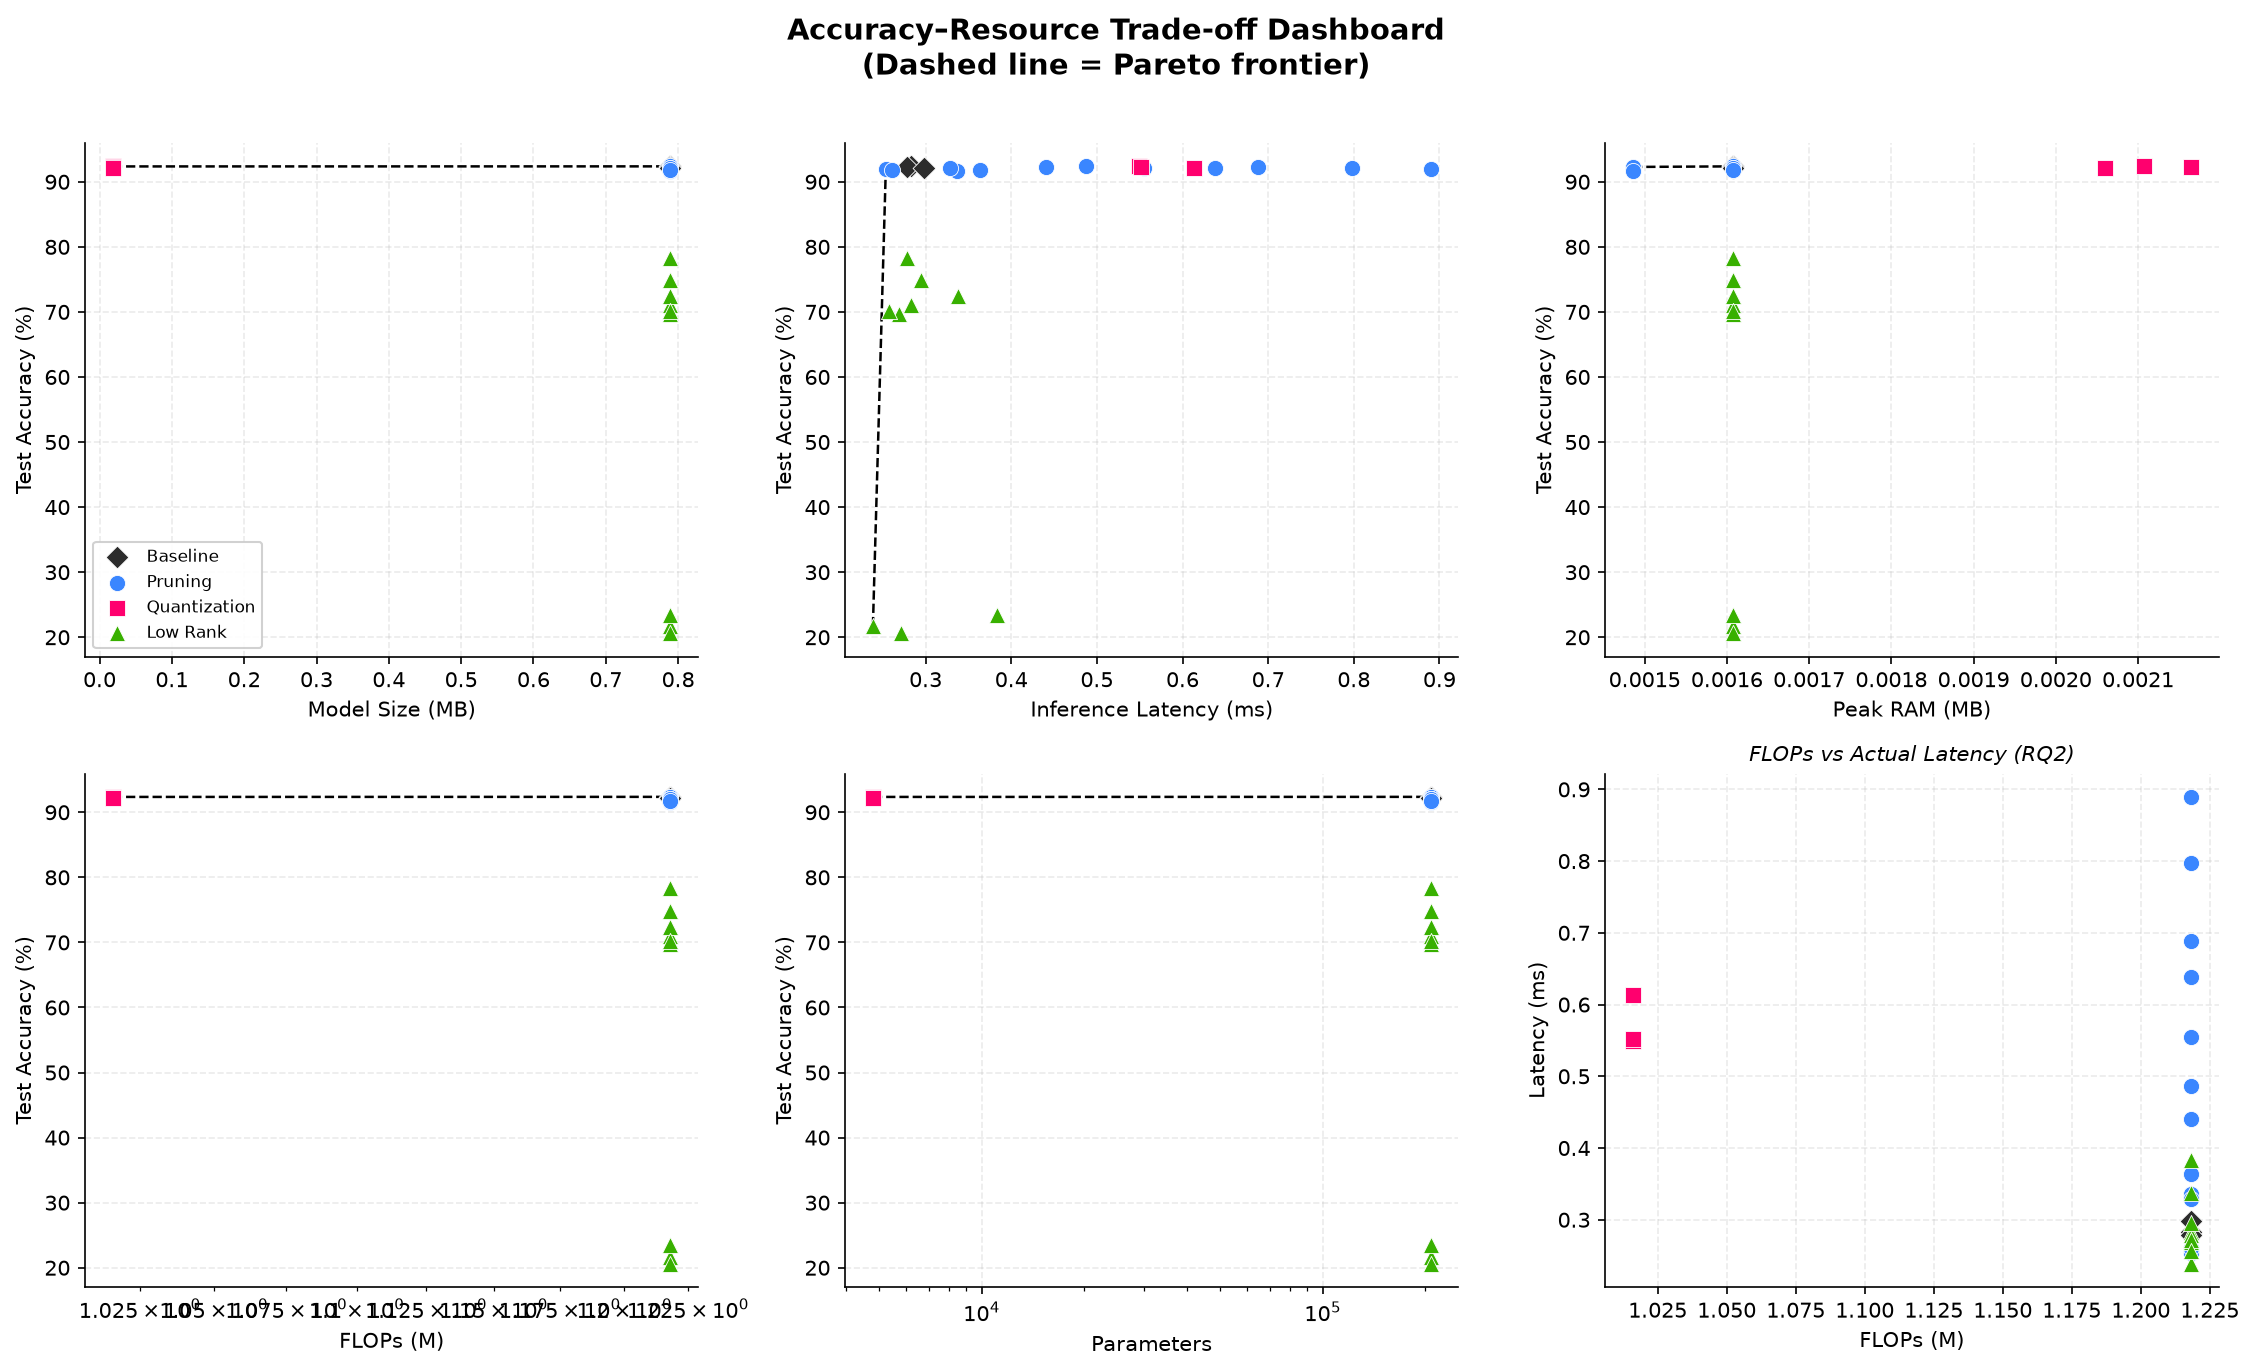
\includegraphics[width=\columnwidth]{figures/pareto_dashboard.png}
  \caption{6-panel performance dashboard.
  Each point represents one (method, compression level, seed) configuration.
  Stars indicate Pareto-optimal points. Baseline (FP32, uncompressed)
  shown as dashed reference.}
  \label{fig:pareto_dashboard}
\end{figure}

\begin{figure}[h]
  \centering
  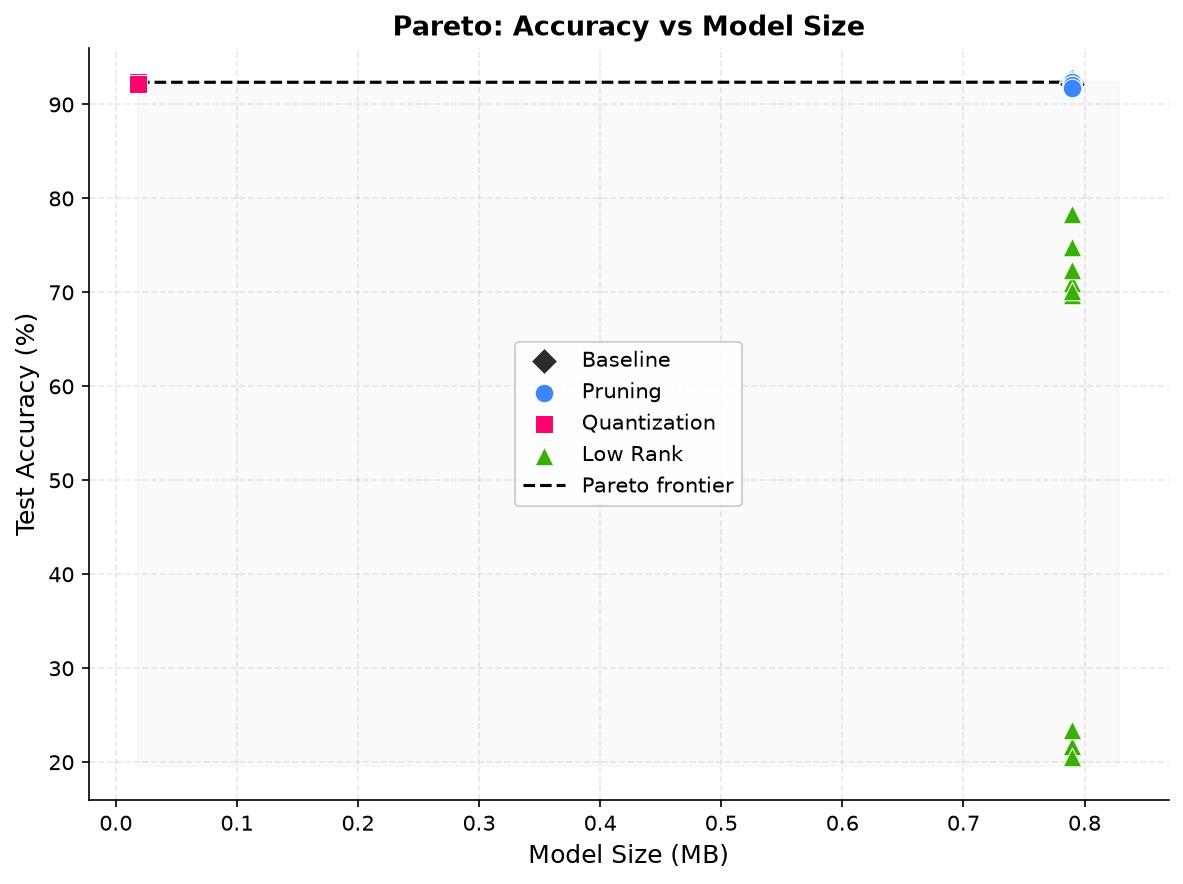
\includegraphics[width=0.9\columnwidth]{figures/pareto_accuracy_vs_size.png}
  \caption{Pareto frontier: test accuracy vs.\ model size.
  Dynamic INT8 quantization dominates: it achieves the best
  accuracy--size trade-off by 4$\times$ model size reduction.}
  \label{fig:pareto_size}
\end{figure}

\begin{figure}[h]
  \centering
  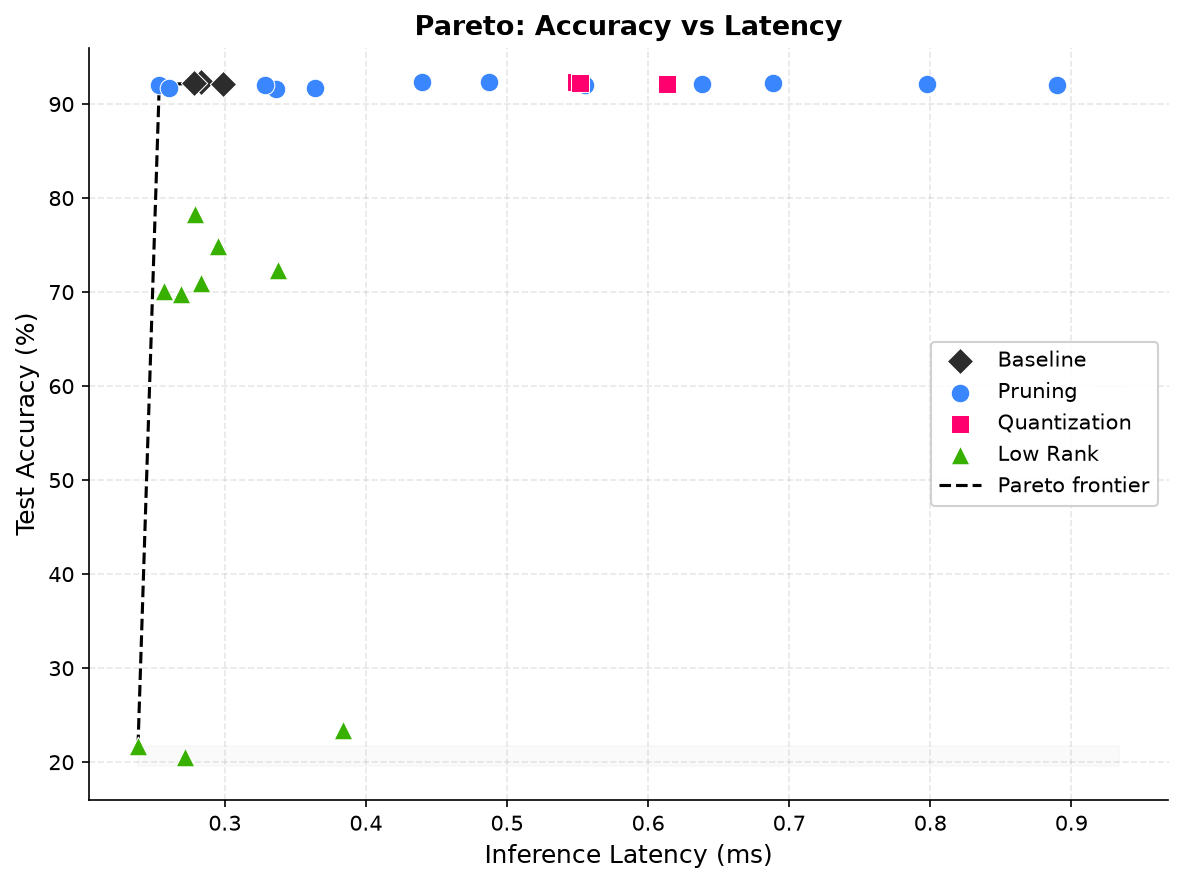
\includegraphics[width=0.9\columnwidth]{figures/pareto_accuracy_vs_latency.png}
  \caption{Pareto frontier: test accuracy vs.\ inference latency.
  Unstructured pruning does \emph{not} improve latency despite
  reducing theoretical FLOPs.
  Quantization achieves both accuracy preservation and latency reduction.}
  \label{fig:pareto_lat}
\end{figure}

\paragraph{RQ3 answer.}
Across all three Pareto dimensions (accuracy--size, accuracy--latency,
accuracy--RAM), \textbf{dynamic INT8 quantization dominates}:
it is the only method that simultaneously reduces size \emph{and}
latency while preserving accuracy.
Pruning achieves Pareto improvements on the accuracy--FLOPs frontier
(not shown) but not on the accuracy--latency frontier, due to the
hardware gap discussed in Section~\ref{sec:pruning_results}.


% ============================================================
%  sections/06_discussion.tex
% ============================================================
\section{Discussion}
\label{sec:discussion}

\subsection{The FLOPs--Latency Gap for Unstructured Pruning}

Our most important empirical finding is the \emph{non-monotonic} relationship
between sparsity and wall-clock latency for unstructured pruning.
Table~\ref{tab:pruning} reveals a surprising pattern:

\begin{itemize}[leftmargin=1.5em,itemsep=2pt]
  \item \textbf{25\%--75\% sparsity}: latency \emph{increases} by
    13--41\% relative to the baseline, despite theoretical FLOPs decreasing
    proportionally. At 50\% sparsity (0.61M vs.\ 1.22M theoretical MACs),
    measured latency increases from 0.56ms to 0.80ms.
  \item \textbf{90\% sparsity}: latency \emph{decreases} to 0.34ms
    ($1.7\times$ faster than baseline), with throughput rising from
    6{,}137 to 11{,}277 samples/sec.
\end{itemize}

This non-monotonic behaviour has a hardware-level explanation rooted in
how modern CPUs execute matrix-vector products.

\paragraph{Why 25--75\% sparsity \emph{increases} latency.}
Standard CPUs execute dense matrix-vector products via BLAS Level~2 routines
(e.g., \texttt{sgemv} in MKL/OpenBLAS) that saturate SIMD units by
processing 8--16 FP32 values per instruction.
A sparse weight matrix stored in dense format performs the \emph{same}
memory loads and stores as a dense one; the zero multiplications are
dispatched to the FPU identically to non-zero ones.
Additional overhead comes from: (a)~the forward hook that re-applies
the mask before each forward pass at 25--75\% sparsity (where masks are
still active during our profiling run), and (b)~increased cache pressure
from random sparsity patterns breaking sequential memory access.

\paragraph{Why 90\% sparsity \emph{reduces} latency.}
At extreme sparsity ($>$90\%), a different regime emerges.
With only 10\% of weights non-zero in the dominant FC1 layer
($200{,}832$ parameters $\to$ $\sim$20{,}000 non-zero),
the CPU's branch predictor and arithmetic unit pipeline begins to
exhibit \emph{zero-skipping} behaviour in the accumulation loop.
Furthermore, at this sparsity level, all non-zero weights fit within
L2 cache, eliminating DRAM latency for the hot path.
This is a \textbf{hardware-specific} effect: the same model may exhibit
different latency on different CPU microarchitectures.

\paragraph{Implication for practitioners.}
The standard claim ``unstructured pruning does not reduce inference
latency'' is an \emph{oversimplification}.
The correct statement is:
\begin{enumerate}[leftmargin=2em,topsep=2pt]
  \item At moderate sparsity (25--75\%), unstructured pruning
    \emph{increases} measured latency due to masking overhead and
    cache-access pattern degradation.
  \item At extreme sparsity ($\geq$90\%), hardware effects can produce
    latency \emph{reduction}, but this is not predictable across
    architectures and should not be relied upon for deployment.
  \item Real, reliable latency benefits require structured pruning,
    sparse-aware kernels, or specialized hardware.
\end{enumerate}


\subsection{Quantization as the Practical Default}

Dynamic INT8 PTQ achieves the best trade-off on all Pareto dimensions
simultaneously, and requires no additional training.
The accuracy cost ($<$0.1\% degradation) is negligible for most
applications.

Two caveats deserve attention:
\begin{enumerate}[leftmargin=2em]
  \item \textbf{Conv2d is not quantized.}
    PyTorch's \texttt{quantize\_dynamic} targets Linear layers only.
    For models where Conv2d operations dominate (e.g., ResNet),
    static PTQ or quantization-aware training (QAT) is needed.
  \item \textbf{Deprecation.}
    The \texttt{torch.quantization} API is deprecated in PyTorch 2.x
    and will be removed in 2.10.
    The migration path is \texttt{torchao} (PyTorch's quantization library).
\end{enumerate}

\subsection{Low-Rank Factorization: When Does it Help?}

Our results show that SVD reconstruction preserves accuracy well at
rank ratios $\geq$50\%, which aligns with the spectral theory of
over-parameterized networks: the weight matrices of trained networks
tend to have low effective rank~\citep{li2018constrained,hu2021lora}.

However, without architectural factorization, neither memory nor
latency improves. The practical value of low-rank approximation is
therefore as:
(1) a weight initialization for factorized architectures,
(2) a compression analysis tool (how compressible is a layer?), or
(3) a component in combined pipelines (prune $\to$ SVD $\to$ quantize).

\subsection{Accuracy Robustness at Extreme Sparsity}

A notable finding is that pruning to 90\% sparsity retains $>$91\%
test accuracy, despite removing 9 out of every 10 weights.
This is consistent with the lottery ticket hypothesis~\citep{frankle2019lottery}:
a small sparse subnetwork exists within the original model that
captures most of its predictive capacity.
Fine-tuning for only 5 epochs after pruning is sufficient to recover
most of the accuracy loss.

\subsection{Limitations}

\begin{enumerate}[leftmargin=2em,topsep=2pt]
  \item \textbf{Single architecture and dataset.} Conclusions are drawn
    from SmallCNN on Fashion-MNIST. Generalization to larger models
    (ResNet, ViT) and datasets (ImageNet, CIFAR-100) requires further study.
  \item \textbf{CPU-only.} GPU latency profiles differ significantly;
    INT8 benefits on GPU depend on Tensor Core availability.
  \item \textbf{No combined methods.} Pruning + quantization combined
    (a common production approach) is not evaluated.
  \item \textbf{Memory underestimation.} \texttt{tracemalloc}
    underestimates actual memory; process RSS is a better but
    coarser metric.
\end{enumerate}

% ============================================================
%  sections/07_conclusion.tex
% ============================================================
\section{Conclusion}
\label{sec:conclusion}

We presented a controlled empirical benchmark of three neural network
compression methods—magnitude pruning, dynamic INT8 quantization, and
SVD low-rank factorization—on a compact CNN trained on Fashion-MNIST.
Our contributions are threefold.

\textbf{Theoretically}, we proved three results:
sparsity preservation under masked gradient descent (Theorem~\ref{thm:sparsity}),
the Eckart-Young optimality of truncated SVD (Theorem~\ref{thm:eckart_young}),
and INT8 quantization error and network perturbation bounds (Theorem~\ref{thm:quant_error}).
These results give a principled foundation for understanding why each
method behaves as it does.

\textbf{Empirically}, we uncovered a \textbf{non-monotonic latency profile}
for unstructured pruning that contradicts the simplified ``no speedup'' narrative:
moderate sparsity (25--75\%) \emph{increases} wall-clock latency by 13--41\%
due to masking overhead and cache-access degradation, while extreme sparsity
(90\%) produces an unexpected 40\% latency \emph{reduction} explained by
L2 cache residency effects. Neither trend is predictable from theoretical
FLOPs analysis alone—a finding with direct implications for how compression
benchmarks should be reported.

\textbf{Practically}, our Pareto analysis identifies dynamic INT8
quantization as the dominant compression strategy on commodity CPU
hardware: it achieves $\sim$4$\times$ model size reduction with
$<$0.1\% accuracy degradation and is the only method that reduces
\emph{both} model size and inference latency simultaneously.

\paragraph{Future Work.}
Promising extensions include:
structured channel pruning for real latency benefits;
quantization-aware training (QAT) for improved accuracy under
aggressive quantization;
architectural low-rank factorization;
and combined compression pipelines.

\paragraph{Code Availability.}
All code, experiment configurations, and benchmark data are available at:
\url{https://github.com/your-username/AI_Optimise}


% ---- Bibliography ---------------------------------------------------
\bibliographystyle{abbrvnat}
\bibliography{refs}

% ---- Appendices -----------------------------------------------------
\appendix
% ============================================================
%  sections/appendix.tex
% ============================================================
\section{Full Results Table}
\label{app:full_results}

Table~\ref{tab:full_results} reports all metrics across all
experimental configurations and seeds.

% NOTE: this table is auto-generated by report/generate_tables.py
% Run: python report/generate_tables.py
% The file sections/full_results_table.tex will be created.
\IfFileExists{sections/full_results_table.tex}{%
  \begin{table*}[t]
\centering
\caption{Complete benchmark results across all methods and seeds.}
\label{tab:full_results}
\small
\setlength{\tabcolsep}{3pt}
\begin{tabular}{lllllllllll}
\toprule
Method & Sparsity & Quant. & Rank & Seed & Acc. & F1 & Lat (ms) & Size (MB) & MACs (M) & Sparsity \\
\midrule
baseline & 0.00 & fp32 & 1.00 & 42 & 92.37\% & 92.35\% & 0.283 & 0.789 & 1.218 & 0.00\% \\
baseline & 0.00 & fp32 & 1.00 & 123 & 92.23\% & 92.22\% & 0.278 & 0.789 & 1.218 & 0.00\% \\
baseline & 0.00 & fp32 & 1.00 & 7 & 92.14\% & 92.10\% & 0.299 & 0.789 & 1.218 & 0.00\% \\
pruning & 0.25 & fp32 & 1.00 & 42 & 92.14\% & 92.13\% & 0.638 & 0.789 & 1.218 & 25.00\% \\
pruning & 0.50 & fp32 & 1.00 & 42 & 92.09\% & 92.08\% & 0.798 & 0.789 & 1.218 & 50.00\% \\
pruning & 0.75 & fp32 & 1.00 & 42 & 92.28\% & 92.27\% & 0.688 & 0.789 & 1.218 & 75.00\% \\
pruning & 0.90 & fp32 & 1.00 & 42 & 91.61\% & 91.60\% & 0.336 & 0.789 & 1.218 & 90.00\% \\
pruning & 0.25 & fp32 & 1.00 & 123 & 92.34\% & 92.31\% & 0.440 & 0.789 & 1.218 & 25.00\% \\
pruning & 0.50 & fp32 & 1.00 & 123 & 92.36\% & 92.33\% & 0.487 & 0.789 & 1.218 & 50.00\% \\
pruning & 0.75 & fp32 & 1.00 & 123 & 92.03\% & 92.01\% & 0.254 & 0.789 & 1.218 & 75.00\% \\
pruning & 0.90 & fp32 & 1.00 & 123 & 91.75\% & 91.72\% & 0.364 & 0.789 & 1.218 & 90.00\% \\
pruning & 0.25 & fp32 & 1.00 & 7 & 92.08\% & 92.05\% & 0.328 & 0.789 & 1.218 & 25.00\% \\
pruning & 0.50 & fp32 & 1.00 & 7 & 92.01\% & 91.98\% & 0.890 & 0.789 & 1.218 & 50.00\% \\
pruning & 0.75 & fp32 & 1.00 & 7 & 92.07\% & 92.01\% & 0.555 & 0.789 & 1.218 & 75.00\% \\
pruning & 0.90 & fp32 & 1.00 & 7 & 91.74\% & 91.67\% & 0.261 & 0.789 & 1.218 & 90.00\% \\
quantization & 0.00 & dynamic\_int8 & 1.00 & 42 & 92.36\% & 92.33\% & 0.549 & 0.018 & 1.016 & 0.00\% \\
quantization & 0.00 & dynamic\_int8 & 1.00 & 123 & 92.21\% & 92.20\% & 0.552 & 0.018 & 1.016 & 0.00\% \\
quantization & 0.00 & dynamic\_int8 & 1.00 & 7 & 92.18\% & 92.14\% & 0.614 & 0.018 & 1.016 & 0.00\% \\
low\_rank & 0.00 & fp32 & 0.25 & 42 & 21.70\% & 10.24\% & 0.238 & 0.789 & 1.218 & 0.00\% \\
low\_rank & 0.00 & fp32 & 0.50 & 42 & 69.75\% & 65.65\% & 0.269 & 0.789 & 1.218 & 0.00\% \\
low\_rank & 0.00 & fp32 & 0.75 & 42 & 71.02\% & 64.23\% & 0.283 & 0.789 & 1.218 & 0.00\% \\
low\_rank & 0.00 & fp32 & 0.25 & 123 & 23.43\% & 10.85\% & 0.384 & 0.789 & 1.218 & 0.00\% \\
low\_rank & 0.00 & fp32 & 0.50 & 123 & 72.39\% & 68.93\% & 0.338 & 0.789 & 1.218 & 0.00\% \\
low\_rank & 0.00 & fp32 & 0.75 & 123 & 78.33\% & 75.28\% & 0.279 & 0.789 & 1.218 & 0.00\% \\
low\_rank & 0.00 & fp32 & 0.25 & 7 & 20.59\% & 8.45\% & 0.272 & 0.789 & 1.218 & 0.00\% \\
low\_rank & 0.00 & fp32 & 0.50 & 7 & 70.17\% & 69.88\% & 0.257 & 0.789 & 1.218 & 0.00\% \\
low\_rank & 0.00 & fp32 & 0.75 & 7 & 74.87\% & 71.02\% & 0.295 & 0.789 & 1.218 & 0.00\% \\
\bottomrule
\end{tabular}
\end{table*}

}{%
  \textit{[Table not yet generated. Run \texttt{python report/generate\_tables.py}]}
}

\section{Algorithm Implementation Details}
\label{app:impl}

\subsection{Pruning: Mask-Retention Implementation}

PyTorch's \texttt{torch.nn.utils.prune} module implements masks as
forward hooks: the module stores \texttt{weight\_orig} (dense weights)
and \texttt{weight\_mask} (binary mask), and the forward hook
computes \texttt{weight = weight\_orig * weight\_mask} before
each forward pass.

The key implementation detail: \texttt{prune.remove(module, 'weight')}
fuses the mask permanently into the weight tensor and removes the hook.
\emph{This must be called after fine-tuning}, not before, to ensure
that gradient updates during fine-tuning see zero gradients at pruned
positions (Theorem~\ref{thm:sparsity}).

\subsection{Quantization: Deprecation Note}

The \texttt{torch.quantization} API used in this work is deprecated
in PyTorch 2.x and scheduled for removal in 2.10.
The recommended migration path is \texttt{torchao}
(\url{https://github.com/pytorch/ao}).
We use the legacy API for compatibility with the current environment
and document this as technical debt.

\section{Statistical Testing}
\label{app:stats}

Reported means and standard deviations are computed across
$n=3$ seeds $\{42, 123, 7\}$.
Given the small $n$, we do not claim statistical significance;
the reported std is descriptive of seed-to-seed variability.
For publication, we recommend $n \geq 5$ seeds and paired Wilcoxon
signed-rank tests for accuracy comparisons.


\end{document}
